%% ----------------------------------------------------------------
%% Thesis.tex -- MAIN FILE (the one that you compile with LaTeX)
%% ---------------------------------------------------------------- 

% Set up the document
\documentclass[a4paper, 11pt, oneside]{Thesis}  % Use the "Thesis" style, based on the ECS Thesis style by Steve Gunn
\graphicspath{Figures/}  % Location of the graphics files (set up for graphics to be in PDF format)
% \usepackage[backend=biber,style=apa]{biblatex}
% Include any extra LaTeX packages required
\usepackage[square, numbers, comma, sort&compress,]{natbib}  % Use the "Natbib" style for the references in the Bibliography
\usepackage{verbatim}  % Needed for the "comment" environment to make LaTeX comments
\usepackage[export]{adjustbox}
\usepackage{vector}  % Allows "\bvec{}" and "\buvec{}" for "blackboard" style bold vectors in maths
% \usepackage{caption}
\usepackage{array}
\captionsetup[figure]{font=footnotesize}
\hypersetup{urlcolor=blue, colorlinks=true}  % Colours hyperlinks in blue, but this can be distracting if there are many links.

%% ----------------------------------------------------------------
\begin{document}
\frontmatter      % Begin Roman style (i, ii, iii, iv...) page numbering

% Set up the Title Page
\title  {Pedestrian Path Prediction Using Deep Learning Techniques}

\authors  {\texorpdfstring
            {\href{your web site or email address}{Anjali Sebastian Karimpil\\117220844}}
            {}
            }
\addresses  {\groupname\\\deptname\\\univname}  % Do not change this here, instead these must be set in the "Thesis.cls" file, please look through it instead
\date       {\today}
\subject    {}
\keywords   {}

\maketitle

%% ----------------------------------------------------------------

\setstretch{1.3}  % It is better to have smaller font and larger line spacing than the other way round

% Define the page headers using the FancyHdr package and set up for one-sided printing
\fancyhead{}  % Clears all page headers and footers
\rhead{\thepage}  % Sets the right side header to show the page number
\lhead{}  % Clears the left side page header

\pagestyle{fancy}  % Finally, use the "fancy" page style to implement the FancyHdr headers

%% ----------------------------------------------------------------
% Declaration Page required for the Thesis, your institution may give you a different text to place here
\Declaration{

\addtocontents{toc}{\vspace{1em}}  % Add a gap in the Contents, for aesthetics

I, Anjali Sebastian Karimpil, declare that this thesis titled, `Pedestrian Path Prediction Using Deep Learning Techniques' and the work presented in it are my own. I confirm that:

\begin{itemize} 
\item[\tiny{$\blacksquare$}] This work was done wholly or mainly while in candidature for a degree at this University.
 
\item[\tiny{$\blacksquare$}] Where any part of this thesis has previously been submitted for a degree or any other qualification at this University or any other institution, this has been clearly stated.
 
\item[\tiny{$\blacksquare$}] Where I have consulted the published work of others, this is always clearly attributed.
 
\item[\tiny{$\blacksquare$}] Where I have quoted from the work of others, the source is always given. With the exception of such quotations, this thesis is entirely my own work.
 
\item[\tiny{$\blacksquare$}] I have acknowledged all main sources of help.
 
\item[\tiny{$\blacksquare$}] Where the thesis is based on work done by myself jointly with others, I have made clear exactly what was done by others and what I have contributed myself.

\end{itemize}
 
 
Signed:\\
\rule[1em]{25em}{0.5pt}  % This prints a line for the signature
 
Date:\\
\rule[1em]{25em}{0.5pt}  % This prints a line to write the 
}

\clearpage  % Declaration ended, now start a new page

%% ----------------------------------------------------------------
% The "Funny Quote Page"
\pagestyle{empty}  % No headers or footers for the following pages

\null\vfill
% Now comes the "Funny Quote", written in italics
\textit{``This, right here, is a pretty sweet dissertation''}

\begin{flushright}
% Anjali Karimpil %If the quote is taken from someone, their name goes here
\end{flushright}

\vfill\vfill\vfill\vfill\vfill\vfill\null
\clearpage  % Funny Quote page ended, start a new page
%% ----------------------------------------------------------------

% The Abstract Page
\addtotoc{Abstract}  % Add the "Abstract" page entry to the Contents
\abstract{
\addtocontents{toc}{\vspace{1em}}  % Add a gap in the Contents, for aesthetics

Pedestrian trajectory estimation is an actively researched problem in the field of Computer Vision and Time-series forecasting. In this work, a Recurrent Neural Network with a relatively less frequently used architecture, called Gated Recurrent Units are employed to predict pedestrian trajectory from x, y co-ordinates of the previous.  Edit this

}

\clearpage  % Abstract ended, start a new page
%% ----------------------------------------------------------------

\setstretch{1.3}  % Reset the line-spacing to 1.3 for body text (if it has changed)

% The Acknowledgements page, for thanking everyone
\acknowledgements{
\addtocontents{toc}{\vspace{1em}}  % Add a gap in the Contents, for aesthetics

I would like to express my gratitude to Dr. Gregory Provan, for setting the scene for such an interesting problem, and motivating me throughout my work, by regularly providing me recent papers in the area.

Dr. Ciar\'{a}n Hughes and Jonathan Horgan from Valeo for their inspiration, ideas, and interim reviews, for this project.

Jayadeep Sasikumar, who carried me out through several dark phases, and tried his best to ensure that I write clean, understandable code.

My besties Sherin, Diana and Ramu who were always available on SOS in my moments of frustration.

My roomies and friends - Ashwini, Dhanya, Neeru - who also partook on the same journey and shared their experience and several valuable resources.

My brother for his practical advice from a non-technical perspective.

Zotero and Sharelatex.com for their awesome products, which made writing a breeze.


}
\clearpage  % End of the Acknowledgements
%% ----------------------------------------------------------------

\pagestyle{fancy}  %The page style headers have been "empty" all this time, now use the "fancy" headers as defined before to bring them back


%% ----------------------------------------------------------------
\lhead{\emph{Contents}}  % Set the left side page header to "Contents"
\tableofcontents  % Write out the Table of Contents

%% ----------------------------------------------------------------
\lhead{\emph{List of Figures}}  % Set the left side page header to "List if Figures"
\listoffigures  % Write out the List of Figures

%% ----------------------------------------------------------------
\lhead{\emph{List of Tables}}  % Set the left side page header to "List of Tables"
\listoftables  % Write out the List of Tables

%% ----------------------------------------------------------------
\setstretch{1.5}  % Set the line spacing to 1.5, this makes the following tables easier to read
% \clearpage  % Start a new page
% \lhead{\emph{Abbreviations}}  % Set the left side page header to "Abbreviations"
% \listofsymbols{ll}  % Include a list of Abbreviations (a table of two columns)
% {
% % \textbf{Acronym} & \textbf{W}hat (it) \textbf{S}tands \textbf{F}or \\
% \textbf{LAH} & \textbf{L}ist \textbf{A}bbreviations \textbf{H}ere \\

% }

%% ----------------------------------------------------------------
% \clearpage  % Start a new page
% \lhead{\emph{Physical Constants}}  % Set the left side page header to "Physical Constants"
% \listofconstants{lrcl}  % Include a list of Physical Constants (a four column table)
% {
% % Constant Name & Symbol & = & Constant Value (with units) \\
% Speed of Light & $c$ & $=$ & $2.997\ 924\ 58\times10^{8}\ \mbox{ms}^{-\mbox{s}}$ (exact)\\

% }

%% ----------------------------------------------------------------
% \clearpage  %Start a new page
% \lhead{\emph{Symbols}}  % Set the left side page header to "Symbols"
% \listofnomenclature{lll}  % Include a list of Symbols (a three column table)
% {
% % symbol & name & unit \\
% $a$ & distance & m \\
% $P$ & power & W (Js$^{-1}$) \\
% & & \\ % Gap to separate the Roman symbols from the Greek
% $\omega$ & angular frequency & rads$^{-1}$ \\
% }
%% ----------------------------------------------------------------
% End of the pre-able, contents and lists of things
% Begin the Dedication page

\setstretch{1.3}  % Return the line spacing back to 1.3

\pagestyle{empty}  % Page style needs to be empty for this page
\dedicatory{Dedicated to my parents Sebastian \& Rosamma \ldots}

\addtocontents{toc}{\vspace{2em}}  % Add a gap in the Contents, for aesthetics


%% ----------------------------------------------------------------
\mainmatter	  % Begin normal, numeric (1,2,3...) page numbering
\pagestyle{fancy}  % Return the page headers back to the "fancy" style
\fancyhead{}
\fancyhead[R]{\nouppercase{\textit{\leftmark}}}
\renewcommand\chaptermark[1]{\markboth{#1}{}}
\fancyfoot[C]{\thepage}
% Include the chapters of the thesis, as separate files
% Just uncomment the lines as you write the chapters

% \pagestyle{empty}
\chapter{Introduction}

Scene understanding, tracking of moving objects, and moving object anticipation are key aspects in the area of Computer Vision. Anticipation of moving objects is an actively researched problem across domains such as robotics, autonomous vehicles, augmented reality, and surveillance.

In an autonomous driving setting, identifying both vehicle and pedestrian intent and predicting the next position helps in taking appropriate actions to avert collision. It is also important in order to maintain safe distances from moving objects. It also enables rational decision-making with respect to all objects in the surrounding area. Even at slow driving speeds of 30 to 40 km per hour, anticipating positions in the next 1 to 2 seconds are useful in making safe driving decisions. Pedestrian path prediction is currently used Advanced Driver Assisted Systems (ADAS) to alert drivers of Vulnerable Road Users (VRUs).

Pedestrian path prediction is a highly challenging area as it is dependent on the behaviour of pedestrians, and pedestrian movement can be highly difficult to predict due to the highly dynamic nature of humans. People may start walking, stop or start running abruptly, and these actions might not be predictable based only on visual clues. 
However, with  improved understanding of context, and feeding details of the surrounding environment, it is envisioned to have a better understanding of human movement in a traffic setting. This would mean creation of a lot of hand-crafted inputs as features. However, with the advent of deep learning, it is hoped that the step of feature engineering can be skipped, so that the algorithm auto-detects features. This work aims at producing a deep learning model to predict pedestrian trajectory, panning out to in the future to be able to incorporate multiple useful data sources. 

Path and trajectory are used interchangeably and mean the same in this work.

\section{Objective}

To predict pedestrian's future trajectory based on cues and information from the current frames. 

\section{Outline}
This dissertation is structured in the following manner. Chapter 1 gives a brief introduction of the problem we are trying to solve and its relevance today. It also gives a background of Deep Learning, so that the reader is familiar with the technique to be adopted in this work. Chapter 2 presents a review of the works related to this problem. Chapter 3 states the problem specifically w.r.t the dataset, and establishes evaluation metrics that will be used for defining the success of the experiment. Chapter 4 details the experimental setup and the describes the dataset to be used. Chapter 5 details the results of the experiments and discussion.

% Write this portion after completion. Should give an overview of this document from this point. refer %https://www.ias.informatik.tu-darmstadt.de/uploads/Theses/HajiGhasemi_MScThesis_2013.pdf





\section{Deep Learning}
\subsection{Background and History}
Deep learning is a field that came into being with the idea of understanding how the human brain learns information and be able to extend that to computers.
The first implemented work in the field of deep learning was in the work of \citet{ivakhnenko_cybernetic_1973}.
Deep learning is a data intensive task, and performs better on very large datasets, and expensive computation. Among the first applications of Deep Learning, recognition of handwritten zipcodes done by Yann LeCunn in 1989 in \cite{lecun_backpropagation_1989} is most popular. While the algorithm worked, it took 3 days for training the algorithm.
With the increase of more computationally powerful machines, more and more experiments with Deep Learning were performed, and now Deep Learning is a part of many state-of-the-art applications, across different domains\cite{sak_fast_2015}\cite{deng_deep_2013}\cite{li_constructing_2014}. Deep Learning rose to popularity in the years following 2011-2012, with its employment in the field of computer vision for object detection. In October 2012, a paper by Ciresan et al, demonstrated in the leading CVPR (Computer Vision and Pattern Recognition) conference  how incorporating max-pooling into Convolutional Neural Networks (CNNs) could break multiple benchmarks, and this saw the rise in popularity of Deep learning in research work. Following this, CNNs were successfully used in different image recognition challenges such as the ImageNet\cite{deng_imagenet:_2009}, Pascal VOC\cite{everingham_pascal_2010} and COCO\cite{lin_microsoft_2014} Challenges.

\subsection{Neural Networks}
Deep learning is a subset of Machine Learning, where neural networks are used. 
A simplistic view of Deep Learning algorithm is to consider it as an optimisation of certain parameters with respect to some constraints. The constraints are called losses or costs in the Deep Learning setup. The optimum value of the parameter is that value that minimises cost. Let's consider a situation where we are given an input variable \(x, \) and target variable y. The goal of the Deep Learning algorithm is to find a mapping \(f^*\), taking in \(x, \) and some parameters \((W, b)\), that correctly maps a given input variable \(x \) to the output \(y \), and gives the lowest value of Loss. The loss is the dissimilarity between the actual y, and the predicted output \(\hat{y}\), and is defined differently depending on the problem.

The difference between deep learning and other traditional machine learning applications is that the mapping that is to be learned, \( f^* \), may be a combination of multiple intermediate functions that are applied to intermediate inputs, and these are not explicitly defined by the programmer. The combination of different functions helps in building flexible decision-making algorithms. Here "flexible" means curved/ complicated decision boundary. The addition of multiple functions is done by having multiple layers with intermediate outputs. These layers is what lends deep learning its name. The presence of more layers makes a network deeper.
In a more formal specification of deep learning, is a complex representation of multi-level functions, modelled using neurons. A neuron is one operation performed on the input data. 


\begin{figure}
    \centering
    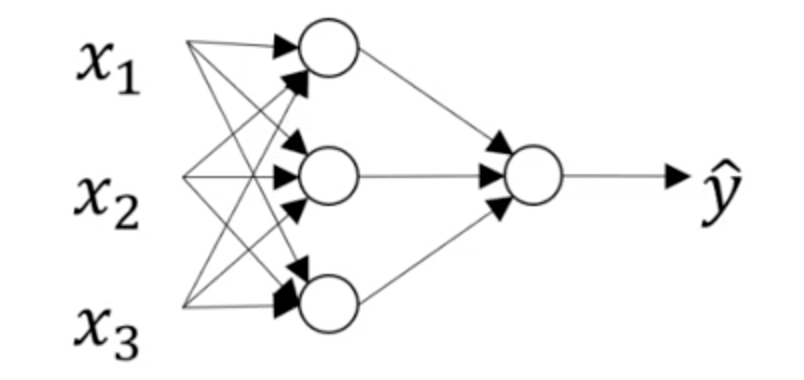
\includegraphics[height=0.15\paperheight]{Figures/nn_simple.png}
    \caption[A basic Neural Network diagram]{Simple Neural Network with 3 input variables predicting target variable y
    \cite{noauthor_neural_nodate}}
    \label{fig:NN_diagram}
\end{figure}

To give a more formal representation, we illustrate this by means of an example. We are given three input variables, and need to find the mapping to a variable, \(y\). Figure \ref{fig:NN_diagram} shows a neural network with 2 layers for this problem.  The number of layers is a tune-able parameter, and depends on the problem. Each layer has weights associated with it. These weights decide the relative importance to be given to each input at that layer. The problem is to find the optimum value of weights to be able to calculate a target variable as accurate as possible from the given input. It is represented by 2 equations:
\[z^{[1]}=W^{[1]}x+b^{[1]}\]
\[a^{[1]}=g(z^{[1]})\]
\[z^{[2]}=W^{[2]}x+b^{[2]}\]
\[a^{[2]}=g(z^{[2]})\]
where X is the matrix of inputs. W is a matrix of weights, and b is a bias vector. This can be vaguely equated to the linear regression equation \(y=mx + c\). The operations above are matrix multiplication and addition operations. Bias can be interpreted as the intercept in the linear regression equation. \(g\) is the called the activation function, and can be a any one of a \(sigmoid, tanh, reLU\) functions. \(a\) is called the activation - more specifically \(a^{[1]}\) is called the activation of the first layer. The activation of the last layer is the output of the neural network, and this is the calculated value of target, given the input. 

Thus, the parameters that need to be optimised are \(W\) and \(b\). There are various algorithms that can be employed to find the optimal value, the most common being back-propagation, a method of taking derivatives, and propagating the error through the network, and making adjustments to the parameters to arrive at the optimal value. Back-propagation is also known by the name of 'Gradient Descent'. The exact history of who invented it are unclear, however it can be seen as an extension of the famous Newton-Ralphson method. Recently, other variants of the algorithm such as ADAM\cite{kingma_adam:_2014}, RMSProp\cite{noauthor_neural_nodate-1} have been invented, and the choice of an optimisation algorithm is also an element of consideration while building and running Neural Networks. These optimisation algorithms have a parameter called learning rate, that decides how big each learning step needs to be. A value too large or too small will make the algorithm optimisation to take too much time to converge. Other techniques such as normalisation also help in the algorithm to converge faster. 


With a small dataset, deep learning only manages to perform rote learning of a data, and spit out outputs. Hence, when using small datasets, care must be taken to ensure that the algorithm does not do this, as otherwise the algorithm will fail on previously unseen data. This is called 'over-fitting'. In order to mitigate this effect, there are techniques called regularisation used.

The number of layers, number of nodes in a layer, normalisation, regularisation, learning rate are tune-able hyper-parameters in building Neural Networks.



Neural Networks also go by the name of Artifical Neural Networks (ANNs) and Multi-Layer Perceptrons (MLPs).

\subsection{Convolutional Neural Networks (CNNs)}
CNNs are specialised neural networks that are used for processing data that have grid-like topology. Convolutional networks are simply neural networks that use convolution in place of general matrix multiplication in at least one of their layers.

In computer vision problems, images are treated as grids of cells, each having some integer value. For example, in a black-and-white image, values in the cells could be 0 meaning black and 1 meaning white. Similarly, for grey-scale images, the integer value could be used for denoting intensity of brightness.

\begin{figure}
    \centering
    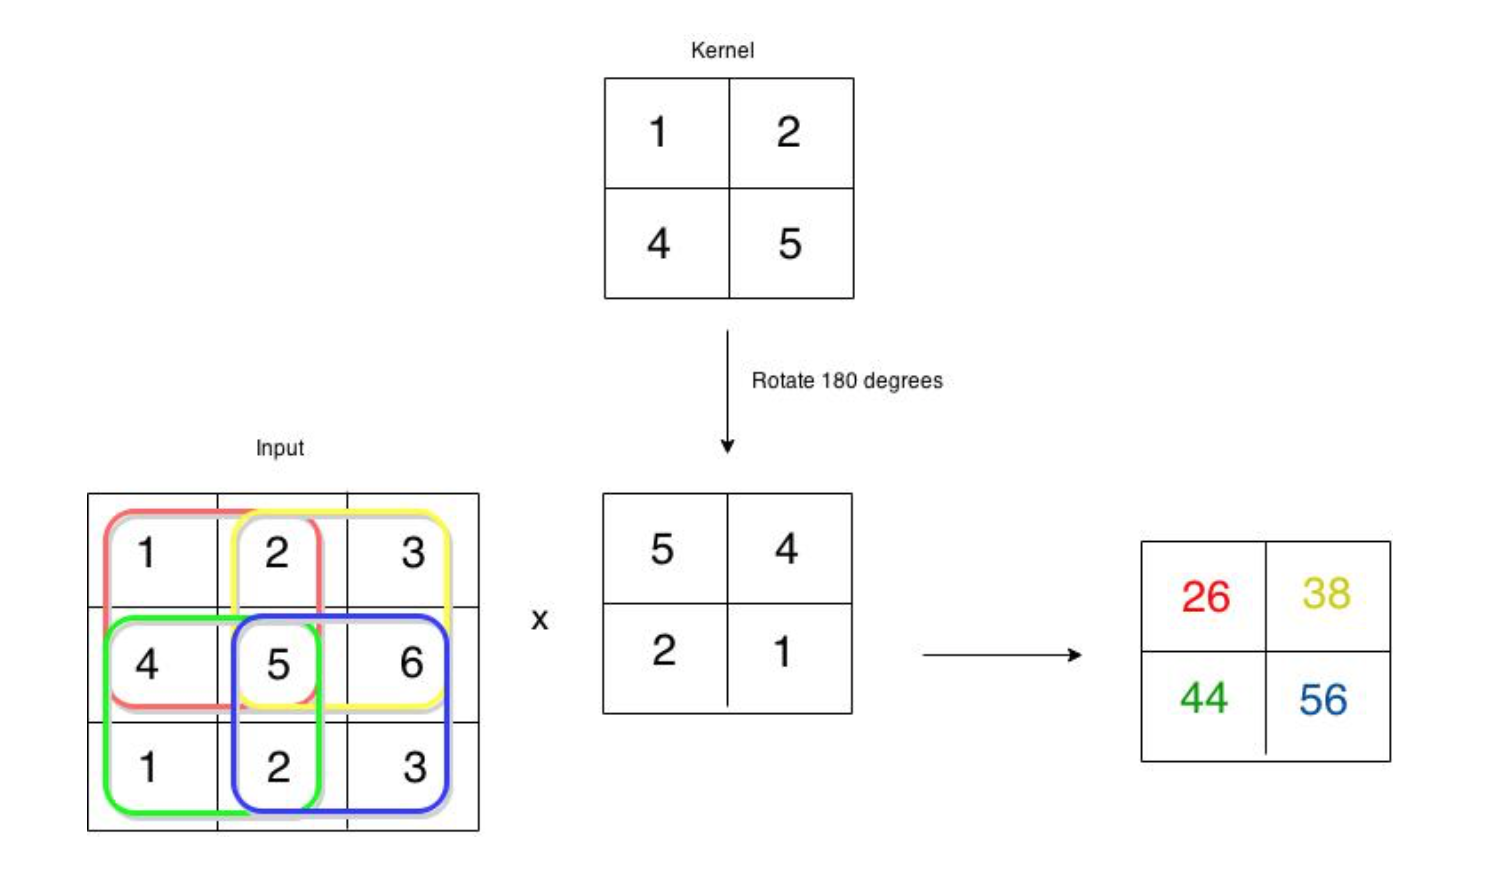
\includegraphics[height=0.2\paperheight]{Figures/CNN_explain.png}
    \caption[Convolution diagram]{Illustration of a convolution
    \cite{noauthor_convolutional_nodate}}
    \label{fig:convolution_diagram}
\end{figure}


A convolution is an operation applied to an image and can be used to identify, extract information or patterns from an image. Figure \ref{fig:convolution_diagram} shows a convolution operation. The \(3 * 3\)  grid is the input image, and the \(2 * 2\) grid is the filter/kernel/convolution - these terms mean the same, and refers to the parameters used to learn the features of the input image. The filter is moved across every \(2 * 2\) combination of boxes, and for each combination, each number is multiplied by the corresponding number on the box, and added up. When a filter is applied to an image it is called 'convolving' the image. Here for the first cell the value is computed as \( (5*1)+(4*2)+(4*2)+(5*1) = 26\).

Figure \ref{fig:convolution_edge_detection} is a simple example of a convolution for edge detection. 


\begin{figure}
    \centering
    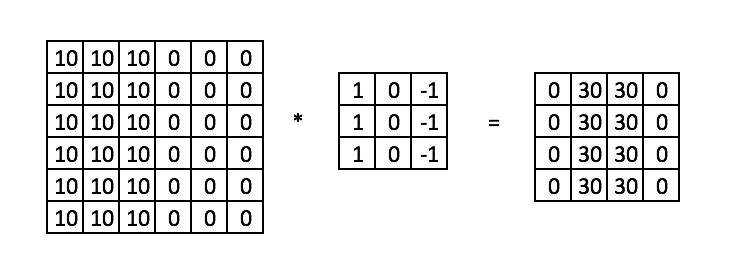
\includegraphics[height=0.15\paperheight]{Figures/cnn_edge_detection.png}
    \caption[Convolution for edge detection]{Convolution for edge detection}
    \label{fig:convolution_edge_detection}
\end{figure}
\subsection{Recurrent Neural Networks (RNNs)}

RNN stands for Recurrent Neural Network. 
RNNs were inspired to be built by the human nature of seeing patterns and being able to extrapolate from it. For example, when humans read a sentence, some words are not read with the same emphasis as others - there are key words that convey ideas.

Keeping this mind, an RNN is a modified version of a Neural Network that can take sequences as input, and learns a feature from all the intermediate inputs into it, and thus learns a sequence. In RNNs, there is parameter sharing across different parts of the sequence, as opposed to plain Neural Networks, and hence they are more suitable for sequential data. Figure \ref{fig:rnn_unit} shows an RNN. We can see from the diagram, there is information passed on from the previous point in the sequence, thus enabling flow of information from one part of the sequence to the next. This is just one RNN unit, and is equivalent to one node of the Neural network representation we have seen earlier. Thus, in addition to back-propagation through layers, there is an added extra functionality of back-propagation through time, within each node in each layer.

\begin{figure}
    \centering
    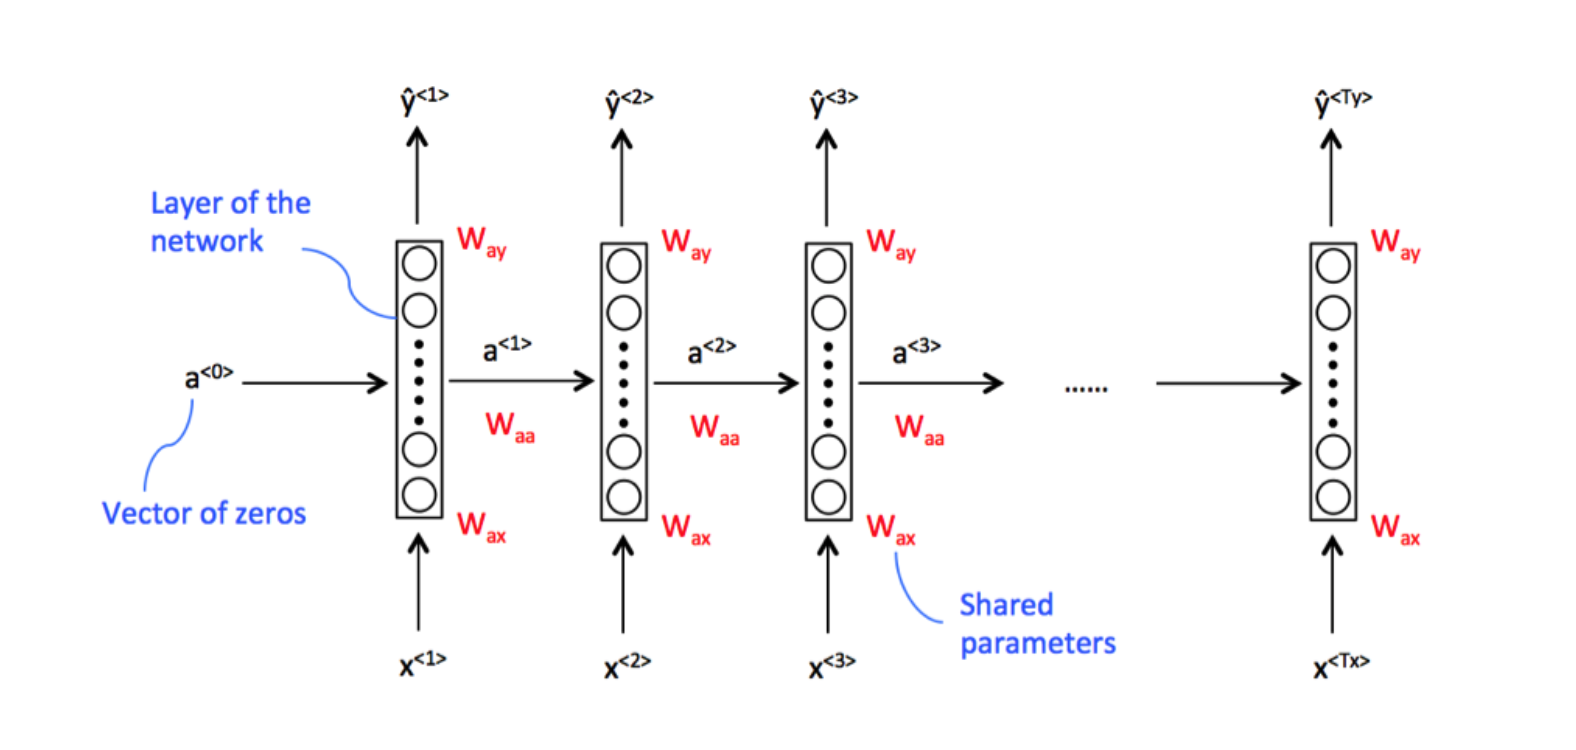
\includegraphics[height=0.2\paperheight]{Figures/rnn_simple.png}
    \caption[Structure of an RNN]{A layer in the RNN\cite{cavaioni_deeplearning_2018}}
    \label{fig:rnn_cell}
\end{figure}

\subsubsection{Simple RNN Unit}

\begin{figure}
    \centering
    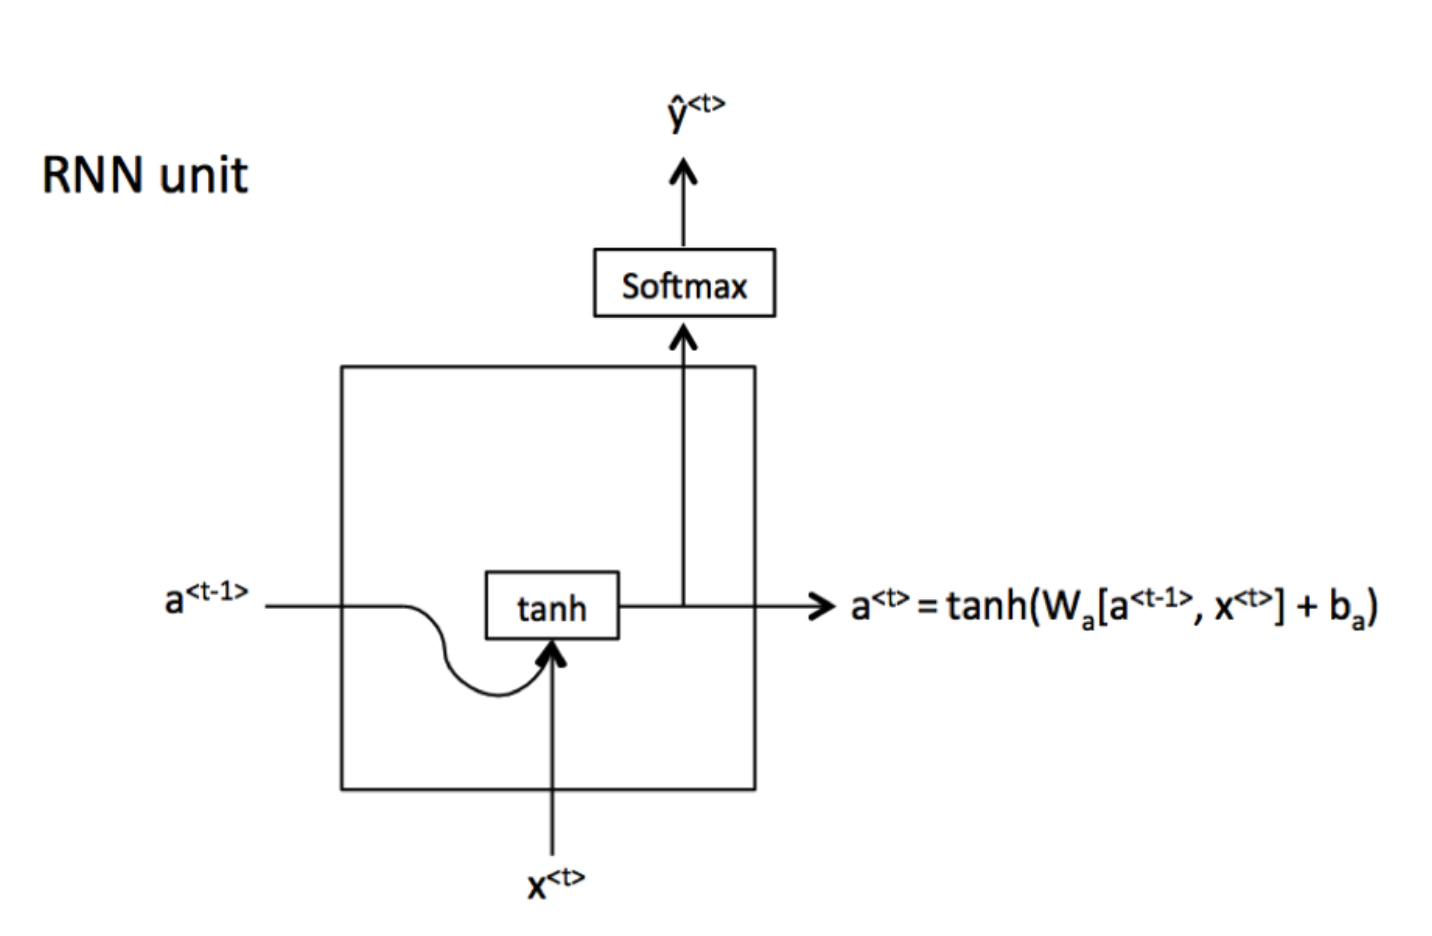
\includegraphics[height=0.2\paperheight]{Figures/RNN_unit.png}
    \caption[An RNN Unit]{RNN unit\cite{cavaioni_deeplearning_2018}}
    \label{fig:rnn_unit}
\end{figure}

In a formal representation of an RNN, the input is X of length \(T_x\). The input at the \(t^{th}\) point is represented by \(x^{<t>}\) and the corresponding output is \(y^{<t>}\). The activation is calculated as:\[a^{<t>}=g(W_{aa}a^{<t-1>}+W_{ax}X^{<t>}+b_a)\]
\(W_{ax}\) is a weight matrix multiplied by another matrix of type \(x\) (the second subscript), i.e., inputs, to get a matrix of the type \(a\) (the first subscript). We simplify the above equation as:
\[a^{<t>}=g_1(W_a[a^{t-1},x^{<t>}]+b)\]
In the above representation, the weight matrices \(W_{aa}\) and \(W_{ax}\) are combined by stacking each other, and similarly \(a^{<t-1>}\) and \(X^{<t>}\) are also stacked. The output is calculated as
\[\hat{y}^{<t>}=g_2(W_{ya}a^{<t>}+b_y)\]
Thus, the activation at every point is a combination of the activation from the previous time step, and of the input value of the current time step. This is how information is passed across time steps in an RNN.
Summarising, and simplifying the notations, we have the following equations that represent an RNN:
\[a^{<t>}=g_1(W_a[a^{t-1},x^{<t>}]+b)\]
\[\hat{y}^{<t>}=g_2(W_{y}a^{<t>}+b_y)\]

For a diagrammatic representation of these equations, refer \ref{fig:rnn_unit}. In this diagram, \(g_1\) is \(tanh\) and \(g_2\) is \(softmax\).




Due to this setup, where the error gradient has to back-propagate through multiple 'cells', it is difficult for the error to reach the initial nodes. This issue is called 'Vanishing gradient'. Due to this problem, the latter parts of the sequence have higher influence on the output when compared to the initial parts of the sequence. In order to counter these issues, modified RNN cells like Gated Recurrent Unit (GRU) and Long Short-Term Memory (LSTM) have been invented. We thus these in detail as this work uses a GRU cell.
\subsubsection{Gated Recurrent Unit (GRU)}
 \begin{figure}[h]
    \centering
    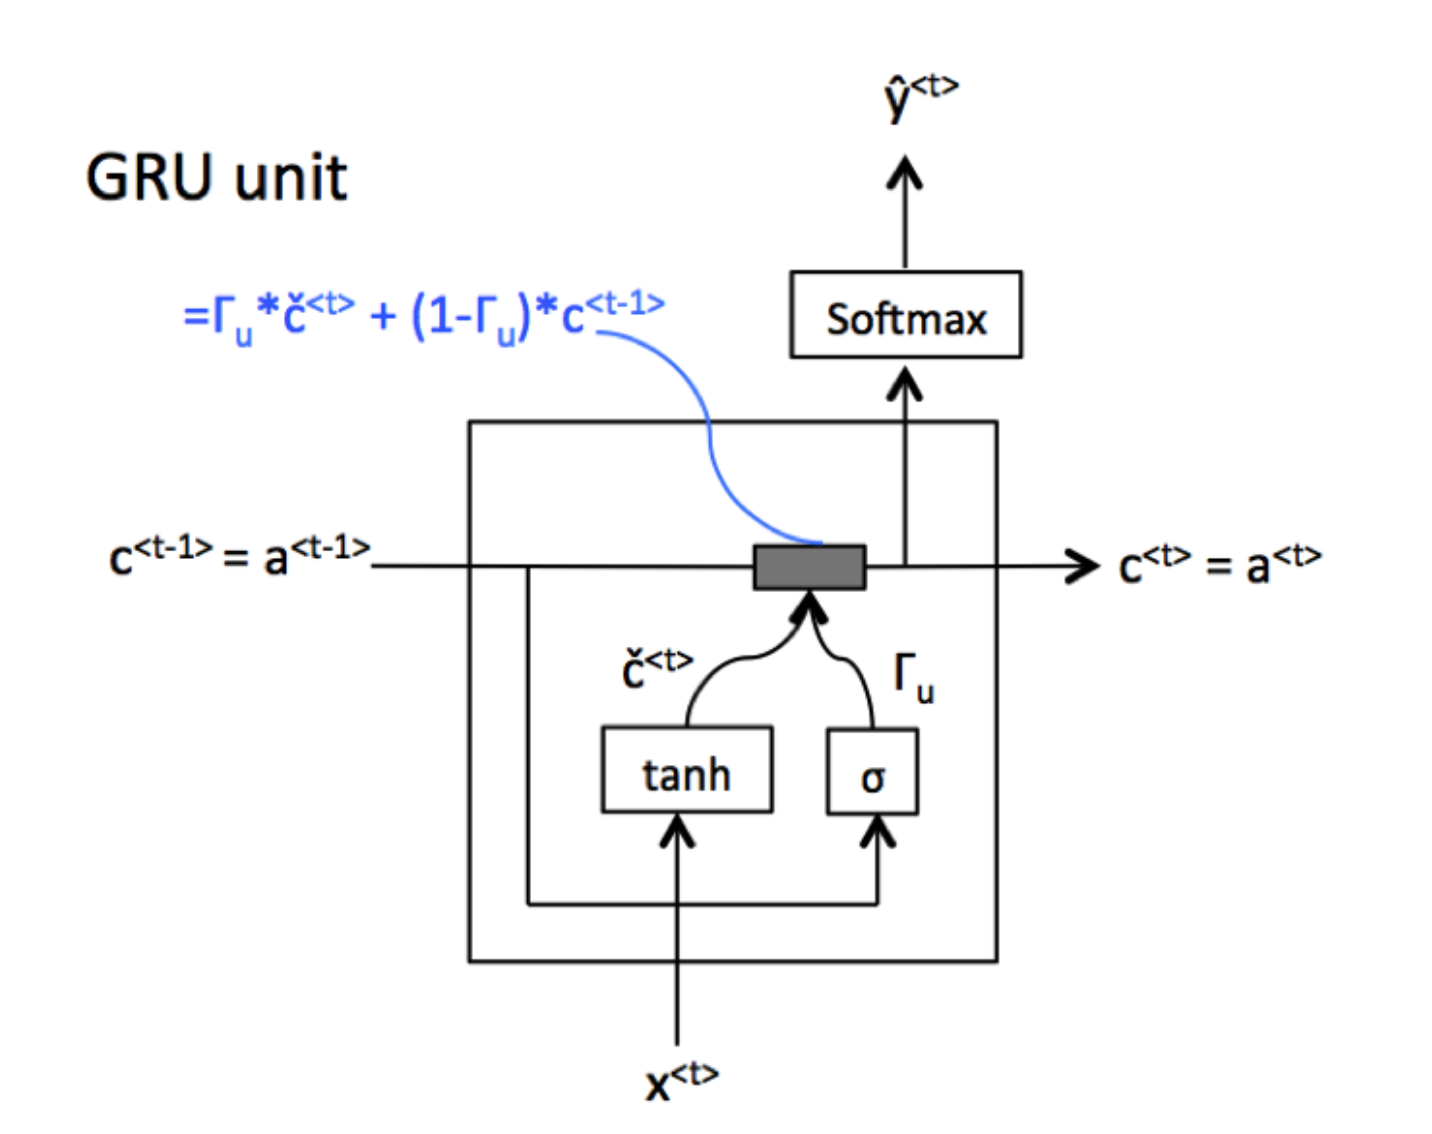
\includegraphics[height=0.25\paperheight]{Figures/GRU_cell.png}
    \caption[GRU Unit]{GRU unit\cite{cavaioni_deeplearning_2018}}
    \label{fig:gru_unit}
\end{figure}
GRUs were introduced in \cite{cho_properties_2014} and \cite{chung_empirical_2014}.
In GRUs, at each time step there is a memory state associated with it, called \(c^{<t>}\). It is initialised with the activation from the previous time step. At every time step, there is a candidate \(\Tilde{c}^{<t>}\) to replace \(c^{<t>}\). It is calculated using the following equation:
\[\Tilde{c}^{<t>}=tanh(W_c[\Gamma_r*c^{<t-1>},x^{<t>}]+b_c)\]
\(W_c\) and \(b\) are parameters. \(\Gamma_r\) is a relevance gate, used for deciding if \(c^{<t-1>}\) is relevant as the next candidate.\(\Gamma_r\) is calculated as:
\[\Gamma_r = \sigma(W_r[c^{<t-1>},x^{<t>}]+b_r)\]
In addition to this, there is an Update gate, \(\Gamma_u\) calculated as:
\[\Gamma_u = \sigma(W_u[c^{<t-1>},x^{<t>}]+b_u)\]
 \(\sigma\) represents the sigmoid function that converts inputs it gets into values between 0 and 1. Thus, the value of \(\Gamma_u\) ranges between 0 and 1. \(\Gamma_u\) decides if we should update the value of \(c^{<t>}\) or not. 
 
 The final update to the memory term at time \(t\) is performed using the following equation:
 \[c^{<t>}=\Gamma_u*\Tilde{c}^{<t>} + (1-\Gamma_u)*{c}^{<t-1>} \]
 Thus, the final value of the memory cell is decided by the update gate, with a certain weightage to the previous memory state, and some to the newly calculated candidate state. Figure \ref{fig:gru_unit} shows a diagrammatic representation of these equations.
 

\subsubsection{Long Short Term Memory (LSTM)}
LSTMs were introduced much before than GRUs, in \cite{hochreiter_long_1997}. LSTMs have a more complicated system of controls when compared to GRUs.
 \begin{figure}[h]
    \centering
    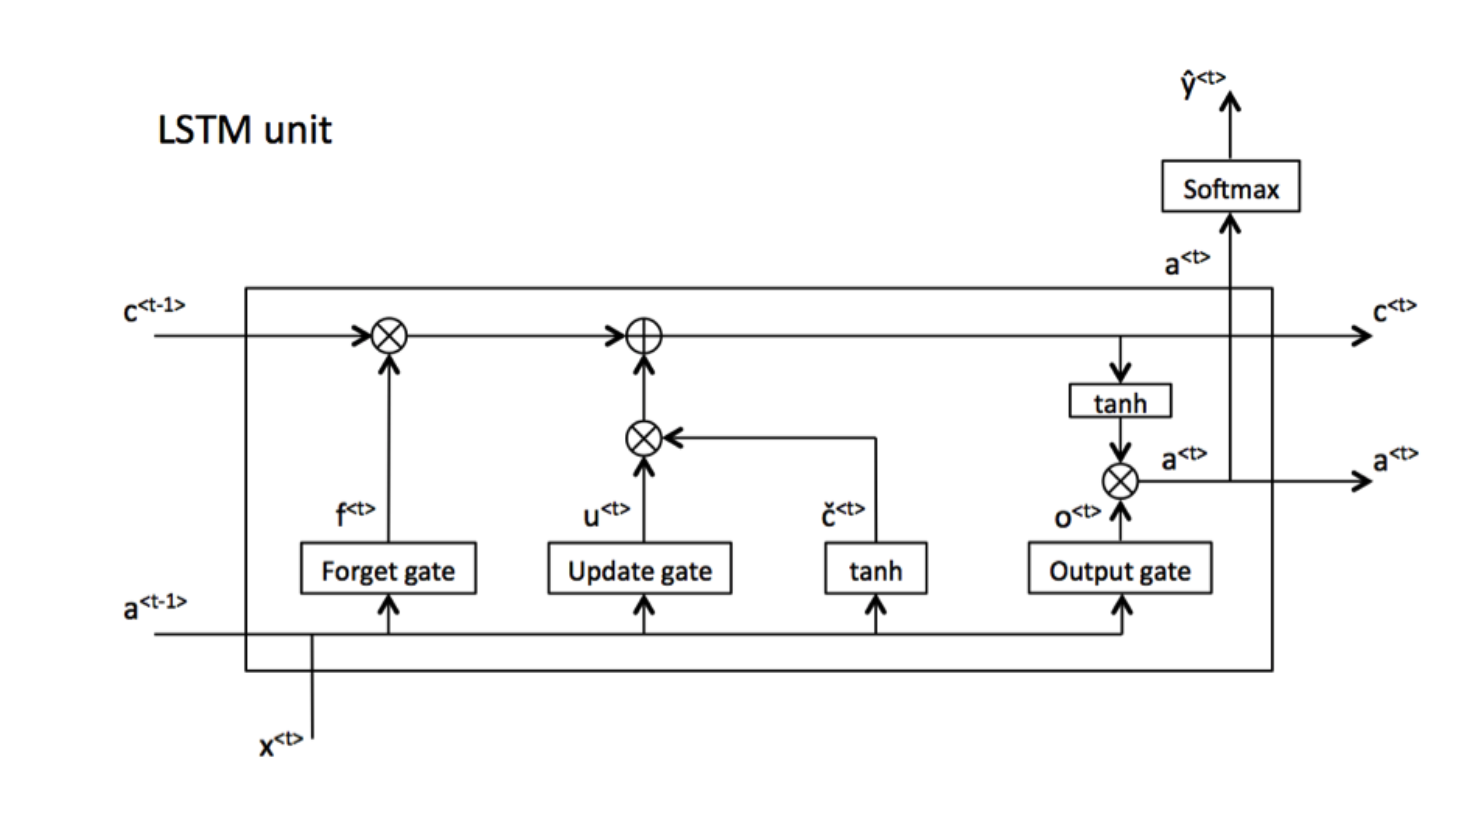
\includegraphics[height=0.25\paperheight]{Figures/LSTM_cell.png}
    \caption[LSTM Unit]{LSTM unit\cite{cavaioni_deeplearning_2018}}
    \label{fig:LSTM cell}
\end{figure}

LSTMs differ from GRUs in the candidate value for the memory cell. Instead of \(c^{<t-1>}\), \(a^<t-1>\) is used.
\[\Tilde{c}^{<t>}=tanh(W_c[\Gamma_r*a^{<t-1>},x^{<t>}]+b_c)\]
Another difference is that, instead of having only 1 update gate, \(\Gamma_u\), there are 2 gates - one for update, and another to forget, \(\Gamma_f\):
\[\Gamma_f = \sigma(W_f[c^{<t-1>},x^{<t>}]+b_f)\]
And another output gate \(\Gamma_o\), calculated as:
\[\Gamma_o = \sigma(W_o[c^{<t-1>},x^{<t>}]+b_o)\]
The new value in the memory cell is calculated using the gates defined above as:
 \[c^{<t>}=\Gamma_u*\Tilde{c}^{<t>} + \Gamma_f*{c}^{<t-1>} \]
 \[a^{<t>}=\Gamma_o*c^{<t>}\]

As LSTMs have many more parameters to be computed, networks with GRUs run faster than LSTMs. As pointed in \cite{chung_empirical_2014}, GRUs and LSTMs perform equally well, and it has not been proved that any one is superior. Hence in this work, we opt for a GRU unit,as it provides almost the same.

Given that RNNs are more appropriate for sequence data, and the problem we are trying to solve is a sequence of pedestrian positions, we will employ RNNs for pedestrian trajectory estimation. As GRUs and LSTMs are equally popular, and no unit has been proved to be superior compared to the other, a simple GRU unit will be used in this work. % Introduction

\chapter{Related Work }

A literature survey of the area was conducted, and we discuss the same in this section.

\section{Traditional methods for pedestrian trajectory estimation}
A popular choice for pedestrian state estimation are traditional time-series methods such as Bayesian filters and Kalman filters. Till today, the benchmark considered is the Kalman filter with an underlying Bayesian model.

In the work of \cite{hutchison_pedestrian_2013}, a comparative study of Bayesian filters were implemented, and a Kalman filter taking into consideration a Constant Velocity (CV) model for recursive state estimation was concluded as the best when compared with other complex Interacting Multiple Model Kalman Filter. Other works such as \cite{keller_will_2014}, investigate the performance of modelling trajectory as Gaussian processes, combined with feeding in features of scene flow and motion features are able to achieve better accuracy in certain situations like stopping and starting, whereas in a state of constant movement, the Kalman filter appears to be the best. 

For the purpose of this work, we do not go into the details of Bayesian filters, but it is to be born in mind that these filters are still considered a significant benchmark due to its accuracy despite the simplicity of the model. 

\section{Deep Learning for pedestrian trajectory estimation}

\subsection{MLP in pedestrian trajectory estimation}
In \cite{goldhammer_pedestrians_2014}, a vanilla Neural Network with 2 intermediate layers is used for trajectory prediction using a training window of 1s and a prediction window of 2s.The ANN exhibits a better estimate of direction of the walking pedestrian, the effect of which is demonstrated by comparing metrics of prediction at 1.2s and 2.5s. 
The difference in prediction is more pronounced at 2.5s. Overall, the ANN method exhibits a 18\% improvement in accuracy. 

Further work by the same authors in 2015, was based on using Multi-layer Perceptron to learn the appropriate polynomial coefficients to model the trajectory, and use this in a polynomial setup to predict the future trajectory. This technique resulted in a 26\% increase in accuracy, suggesting that the way forward would be to use deep learning in conjunction with a traditional algorithm.

In their follow up work in 2018 \cite{goldhammer_intentions_2018}, build on this to use a method they termed as 'Poly-MLP', where the trajectory prediction is done in 2 steps: in the first step, a neural network classifier is used to classify the pedestrian action into one of several states such as walking, starting, stopping, moving, and a second neural network is used, taking both the state of the walking pedestrian and the polynomial coefficients used to represent the time series, as done in their previous work in \cite{goldhammer_camera_2015}



\subsection{RNNs in pedestrian trajectory estimation}
\subsubsection{In crowd surveillance}
Recently, Recurrent Neural Networks are rising in popularity in the context of sequence generation and prediction. Their expertise with respect to sequences make them a suitable candidate to be used in the area  time series prediction problems, and hence can be applied to the problem of predicting trajectories of pedestrians. 

has been employed to model the future trajectories of pedestrians. In the work of \cite{alahi_social_2016}, human-human interaction of trajectories is modelled using a 'Social' aspect. This models how walking pedestrians might change path to accommodate other pedestrians crossing their paths. Subsequent work to include static obstacles has been done in \cite{varshneya_human_2017} and \cite{bartoli_context-aware_2017} to integrate static obstacles as well in the prediction of the path of a walking pedestrian. This has been extended to include pedestrians in far off vision to also be incorporated in the work of \cite{vemula_social_2017}

As discussed earlier, CNNs work on a grid-like structure. \cite{leibe_pedestrian_2016} models pedestrian trajectories using their displacements across time as a 3-D Volume and this is fed into a Convolutional Neural Network. This is a novel method, and the modelling of trajectories as displacement helps replicate the state-of the-art.


\cite{hasan_mx-lstm:_2018} uses estimated head pose for trajectory prediction in a technique called 'MX-LSTM'. It performs well in cases where the pedestrians are walking faster. The errors are higher when the pedestrian is walking slowly, as the head pose angle detected, does not give an accurate idea of the direction of the walking pedestrian. This might suggest that a combination of an approach of estimating velocity of the walking pedestrian combined with MX-LSTM might give better results.



\subsubsection{In traffic setting}
Recent works such as \cite{bhattacharyya_long-term_2017}, employ RNNs employing an encoder-decoder architecture and incorporate probabilistic parameters in their model, so that each prediction also outputs a confidence of the prediction. This achieves better results compared to the state-of-the-art as it is more robust to mistakes during recursive predictions.

A very recent work, Scene-LSTM \cite{manh_scene-lstm:_2018} has emerged which take into consideration the objects in the scene, achieving 80\% reduction in displacement errors.

\subsection{RNN architecture}

Gated Recurrent Units were introduced in \cite{cho_properties_2014}. Subsequent empirical evaluation done in the work of \cite{chung_empirical_2014} suggest that both GRU and LSTM have similar performance

In the work of \cite{yin_comparative_2017}, it has been demonstrated that RNNs perform much better than CNNs in the case of sequence modelling, and hence RNNs are better suited for the purpose. Hence, in this work, we employ a GRU architecture in RNN to solve the problem of pedestrian trajectory estimation.

 % Literature Review

\chapter{Experiments}

\section{Tools used}

\subsection{Hardware}
Deep learning models were trained on a machine with Intel i7-6800K hexacore CPU with an NVIDIA GPU GTX 1080 GPU. Development was done on my personal laptop, a 2014 MacBook Pro with Intel i5 Core.

\subsection{Deep Learning Framework}
There are many libraries available for implementing neural networks. The most common among them are TensorFlow\cite{noauthor_TensorFlow:_2018}, Keras\cite{noauthor_keras_nodate}, PyTorch\cite{noauthor_pytorch_nodate}, CNTK\cite{noauthor_microsoft_2018}, MXNet\cite{noauthor_incubator-mxnet:_2018}. Due to its heavy popularity in tutorials, I drilled down to choosing between Keras and TensorFlow. Keras is a high-level abstraction, and can be used in combination with either of TensorFlow or Pytorch. Keras is easy to learn for a beginner, and well documented, with many standard networks to be easily implemented with a few lines of code. However, I chose to use TensorFlow, with the notion that I might have to build networks that are much complicated. For more complicated implementations, Keras does not have straightforward solutions, and TensorFlow is recommended. 
Finally, TensorFlow version 1.9 for GPU was used in this work.

Additional requirements for the smooth working of TensorFlow for GPU are CUDA and CuDNN. CUDA version 9.0 and CuDNN version 7.0 were installed on the systems.

\subsection{Language and environment}
R and Python were considered for development. Python 3.5 was used for the project as Python is more efficient when handling large datasets, and better compared to R from a deployment perspective.
Initially, I used Jupyter Notebooks for exploration and development. However, Jupyter prvoed to be inefficient while deploying code, and I shofted to using Python files in a basic code editor, Sublime Text\cite{noauthor_sublime_nodate}. 

\subsection{Version control and Tracking}
In order to keep track of progress and the several version, I used git. In order to facilitate transition between the 2 machines I worked on, I decided to use Github. All the development code is present in \url{https://github.com/pattern-recogniser/pedestrian-trajectory-predictor}


It is evident that there is heavy research being done for trajectory prediction in the domain of crowd forecasting, and subsequently the majority of data sources come from crowd surveillance. 
Several trajectory datasets were considered. However, as it would be best to use a source that would give the most data, I decided to use the dataset from Socially Aware Crowd Forecasting. 
An interesting point to be noted is that in the case of pedestrian trajectory prediction in a traffic setting, there are no benchmark datasets.
\begin{table}[]
\begin{tabular}{|l|l|l|}
\hline
Dataset     & Domain            & \# of pedestrians \\
\hline
ETH**       & Crowd forecasting      & 360          \\
\hline
UCY*        & Crowd forecasting      & 204          \\
\hline
Zara-01*    & Crowd forecasting      & 204          \\
\hline
Zara-02*    & Crowd forecasting      & 207          \\
\hline
Social-LSTM & Crowd forecasting      & 14k          \\
\hline
Poly-MLP    & Pedestrian \& Cyclists & 1068 pedestrian, 464 cyclist trajectories\\
\hline
\end{tabular}
\caption{Datasets considered}
\label{table:dataset_considered}

\end{table}
\section{Experimental Setup}
\section{Dataset}

The dataset used is a set of trajectories collected from a train station from the work of Alahi et al. \cite{alahi_socially-aware_2014}. It consists of 42 million trajectories. 
The data is split across 13 files that are in .csv format, with each file having around <insert number here> number of rows. Each file represents one day's recorded data. The data is sampled at 100 millisecond intervals. Each row in the .csv file is a combination of time-stamp, x-co-ordinate and y-coordinate position in millimetres from the origin, which is the top left of the image. There are on average <insert number here> of pedestrians in each file
\begin{figure}
    \centering
    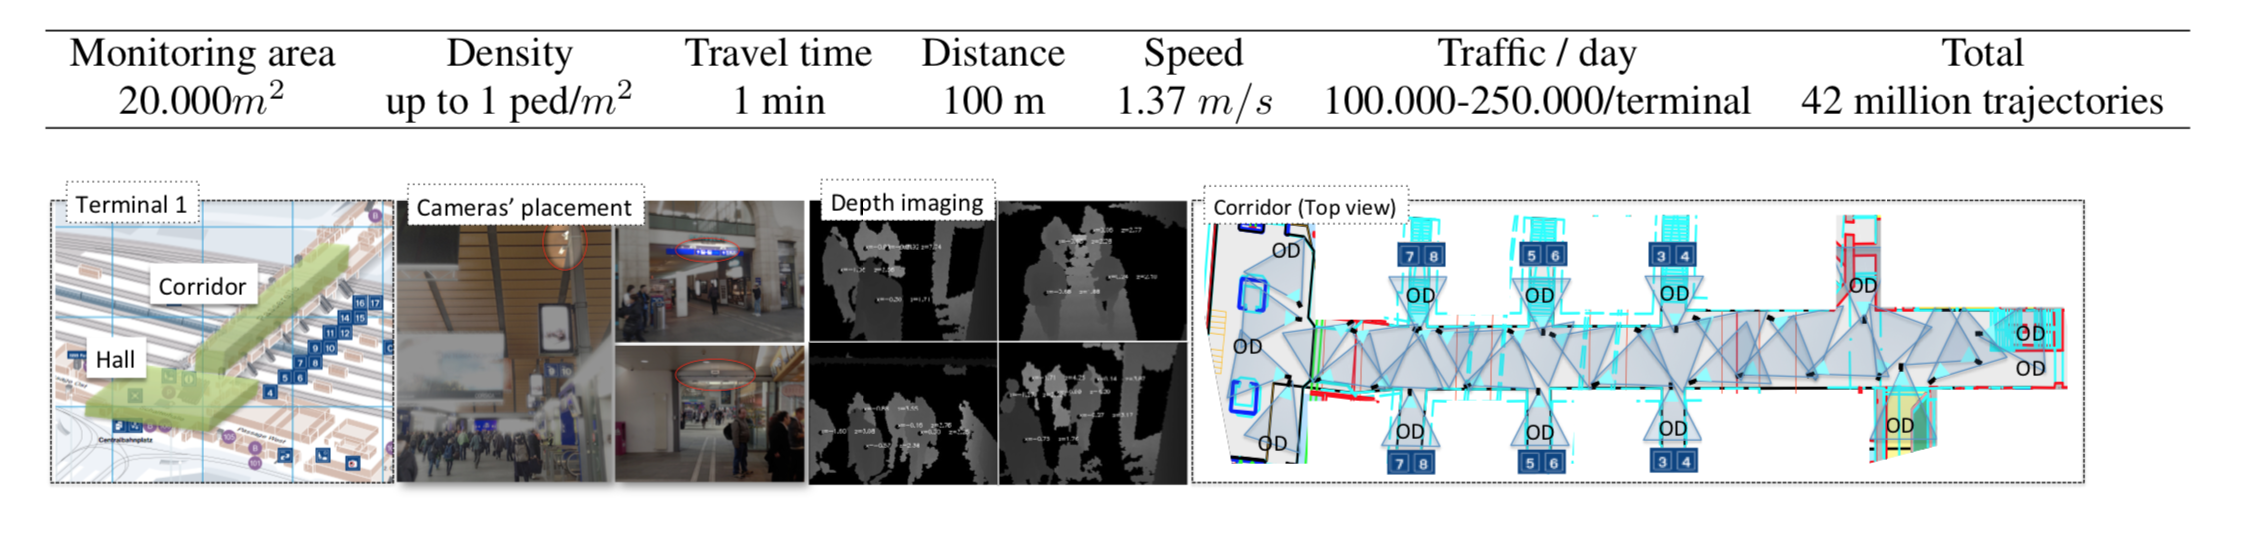
\includegraphics[width=\textwidth]{Figures/Dataset_explanation.png}
    \caption[Key info of Dataset used]{Real-world setup. Top row presents some facts regarding the dataset (values are in average). Bottom row illustrates one of the monitored corridors. More than 30 cameras are deployed in the presented corridor, whereas 132 cameras are deployed in total in 3 corridors, one track, and one large hall. At any given time, the occupancy of the corridor can reach more than one thousand of pedestrians. The label 'OD' represents entry/exit zones }

    \label{fig:dataset_explanation}
\end{figure}

\section{Data Handling}
Data is processed and stored on file as a processed pickle.
Data is read in by keeping only 




\section{Data Cleaning}
\begin{itemize}
    \item Assigning a trajectory ID:
    
    The same pedestrian if observed after a span of 2 minutes is considered as a different trajectory.
    
    \item Removing Outliers:
    
    If consecutive x co-ordinate or y-co-ordinate positions differ by more than 500 millimetres, we consider these as another trajectory. This is equivalent to capping the speed of a walking person to \(5 m/s\)
    
    \item Normalisation
    

\end{itemize}

Data is split into train:test:dev set using a 98:1:1 split.
Final reported metrics are from the test set. Results of loss from the dev set are also reported in this document. However, as a performance metric, only the test set metric is used.









 % Experiments


\chapter{Experiments}

In this chapter, the experimental setup used in this project is detailed.
\section{Tools used}

\subsection{Hardware}
Deep learning models were trained on a machine with Intel i7-6800K hexacore CPU with an NVIDIA GPU GTX 1080 GPU. Development was done on the author's personal laptop, a 2014 MacBook Pro with Intel i5 Core.

\subsection{Language and environment}
R and Python were candidates considered for development. Python 3.5 was used for the project as Python is more efficient when handling large datasets, and better compared to R from a deployment perspective.
Initially, Jupyter Notebooks were used for exploration and development. However, Jupyter proved to be inefficient while deploying code, the code was written and run in Python files developed in a basic code editor, Sublime Text\cite{noauthor_sublime_nodate}. 

\subsection{Deep Learning Framework}
There are many libraries available for implementing neural networks. The most common among them are TensorFlow\cite{noauthor_TensorFlow:_2018}, Keras\cite{noauthor_keras_nodate}, PyTorch\cite{noauthor_pytorch_nodate}, CNTK\cite{noauthor_microsoft_2018}, MXNet\cite{noauthor_incubator-mxnet:_2018}. Due to its heavy popularity in tutorials, Keras and TensorFlow were the major choice to be made. Keras is a high-level abstraction, and can be used in combination with either of TensorFlow or Pytorch. Keras is easy to learn for a beginner, and well documented, with many standard networks to be easily implemented with a few lines of code. However, TensorFlow was chosen for this work with the notion that there might be the need to build networks that are much complicated. For more complicated implementations, Keras does not have straightforward solutions, and TensorFlow is recommended. 
Finally, TensorFlow version 1.9 for GPU was employed in this work.

Additional requirements for the smooth working of TensorFlow for GPU, mentioned in the official TensorFlow documentation age, CUDA and CuDNN. CUDA version 9.0 and CuDNN version 7.0 were installed on the systems.



\subsection{Version control and Tracking}
In order to keep track of progress and efficeintly store several versions, git was used . In order to facilitate transition between the 2 machines that were used, Github was used. All the code developed in this project is present in \url{https://github.com/pattern-recogniser/pedestrian-trajectory-predictor}

\section{Dataset}
From the previous chapter, it is evident that there is heavy research being done for trajectory prediction in the domain of crowd forecasting, and subsequently the majority of data sources come from crowd surveillance. 
Several trajectory datasets were considered. However, as it would be best to use a source that would give the most data, it was decided to use the dataset from Socially Aware Crowd Forecasting. 
An interesting point to be noted is that in the case of pedestrian trajectory prediction in a traffic setting, there are no benchmark datasets.
\begin{table}[h]
\begin{tabular}{|l|l|l|}
\hline
Dataset     & Domain            & \# of pedestrians \\
\hline
ETH**       & Crowd forecasting      & 360          \\
\hline
UCY*        & Crowd forecasting      & 204          \\
\hline
Zara-01*    & Crowd forecasting      & 204          \\
\hline
Zara-02*    & Crowd forecasting      & 207          \\
\hline
Social-LSTM & Crowd forecasting      & 14k          \\
\hline
Poly-MLP    & Pedestrian \& Cyclists & 1068 pedestrian, 464 cyclist trajectories\\
\hline
\end{tabular}
\caption{Datasets considered}
\label{table:dataset_considered}

\end{table}

\subsection{Data Understanding}

The dataset used is a set of trajectories collected from a train station from the work of Alahi et al.\cite{alahi_socially-aware_2014}. It consists of 42 million trajectories. 
The data is split across 13 files that are in .csv format, with each file having around 4 million rows each. Each file represents one day's recorded data. The data is sampled at 100 millisecond intervals. Each row in the .csv file is a combination of time-stamp, x-coordinate and y-coordinate position in millimetres from the origin, which is the top left of the image. There are on average 1000 pedestrians in each file. The total size of the file amounts to 6 GB of data.
\begin{figure}[h]
    \centering
    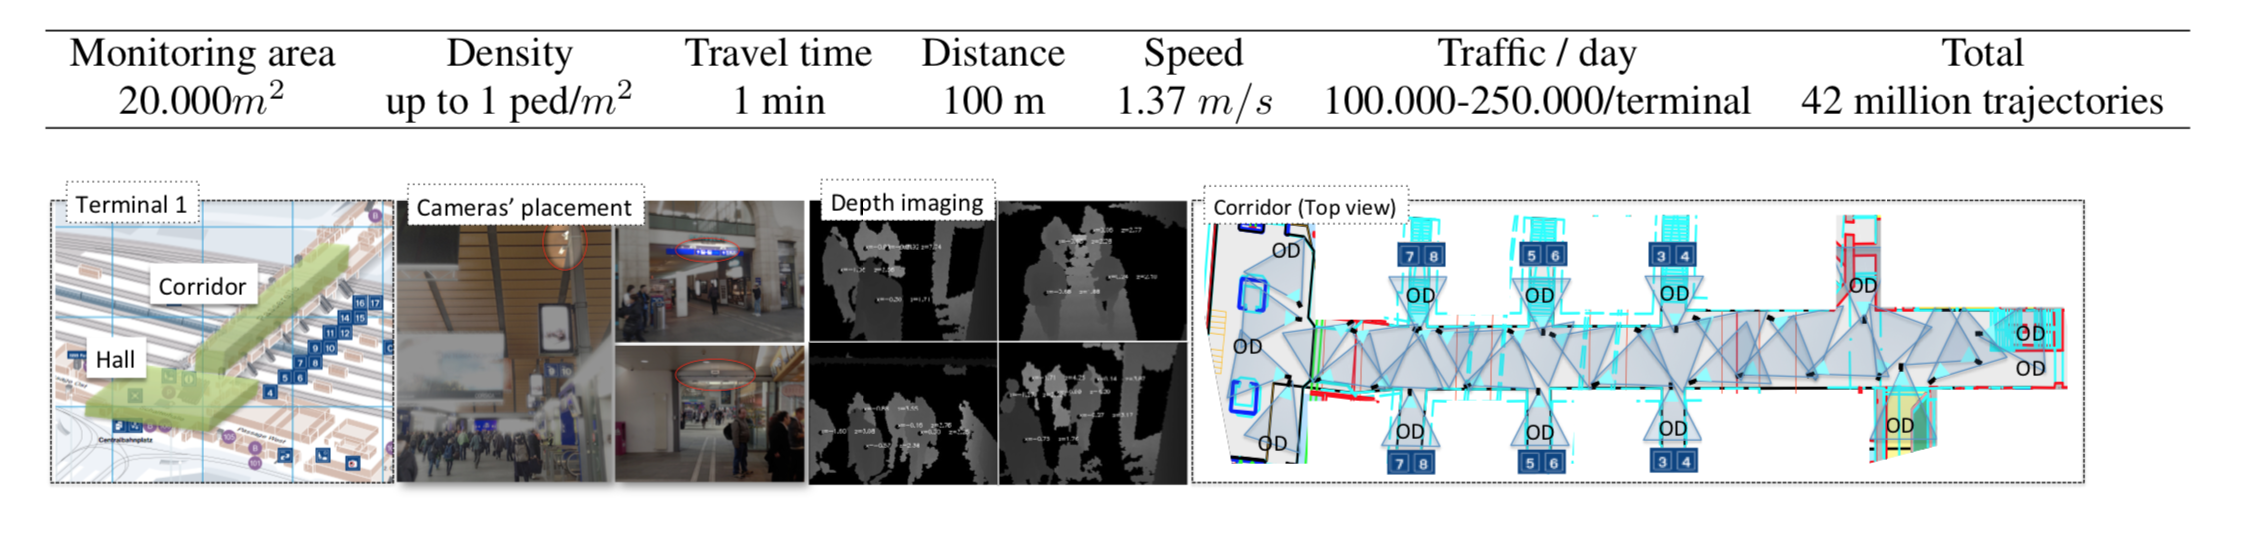
\includegraphics[width=\textwidth]{Figures/Dataset_explanation.png}
    \caption[Key info of Dataset used]{Real-world setup. Top row presents some facts regarding the dataset (values are in average). Bottom row illustrates one of the monitored corridors. More than 30 cameras are deployed in the presented corridor, whereas 132 cameras are deployed in total in 3 corridors, one track, and one large hall. At any given time, the occupancy of the corridor can reach more than one thousand of pedestrians. The label 'OD' represents entry/exit zones \cite{alahi_socially-aware_2014}}

    \label{fig:dataset_explanation}
\end{figure}






\subsection{Data Processing}
\subsubsection{Identifying trajectories}

Each continuous distinct path taken by a pedestrian is identified as a trajectory. Two consecutive positions of the same pedestrian, if observed after a span of 2 seconds are considered belonging to different trajectories.
As the average time difference between consecutive recorded positions of a pedestrian is 100 milliseconds, a threshold of 2 seconds is a conservative one.
Consecutive x or y co-ordinate positions differing by more than 500 millimetres are considered belonging to different trajectories. This is equivalent to clamping the speed of a walking person to \(5 m/s\).
    
\subsubsection{Normalisation of inputs}
In order to speed up the learning algorithm, the input positions have been normalised. The resultant normalised dataset is centred around 0, and has a standard deviation of 1. The minmaxscaler method from sklearn was used to perform normalisation \cite{noauthor_sklearn.preprocessing.minmaxscaler_nodate}.

\subsubsection{Splitting the data}

Data is split into train:test:dev set using a 98:1:1 split. This has been used instead of a standard 70:20:10, as in this case, the data is pretty big, and 1\% of the data would be close to half a million rows. Dev set is another name used for the validation set. Hyper-parameter tuning of the network is done based on performance on the Dev set. Final reported metrics are from the test set. This is to ensure that the performance metric is not specific to the data that we have used for the model, and gives a better measure of the model's performance when it is used for previously unseen data. Results of loss from the dev set are also reported in this document. However, as a performance metric, only the test set metric is used.

\section{Implementation}
\subsection{Data Handling}

As each individual file is big, keeping all the files as a list resulted in Memory error. In order to deal with this, only one file is stored in memory at a time. Each file is read from disk, processed, and finally converted into input format-ready, and then pickled back to disk. When handing data into the network, the data is read from the pickled file on disk, and passed to the network.

\subsection{Network Architecture}
There is one input layer, one hidden layer with 200 RNN units in it, and one output layer. A learning rate of 0.05 was used. Data was fed into the model in a batch of 128. Adam optimiser is used to find the optimal values of parameters.

The observation window considered here is for 1 seconds, and the prediction window is 3 seconds. This has been used keeping in mind that at average driving speeds, the maximum observation time would be 1 second, and predicting 3 seconds ahead will be beneficial for the driver alert mechanism.
\begin{figure}[ht]
    \centering
    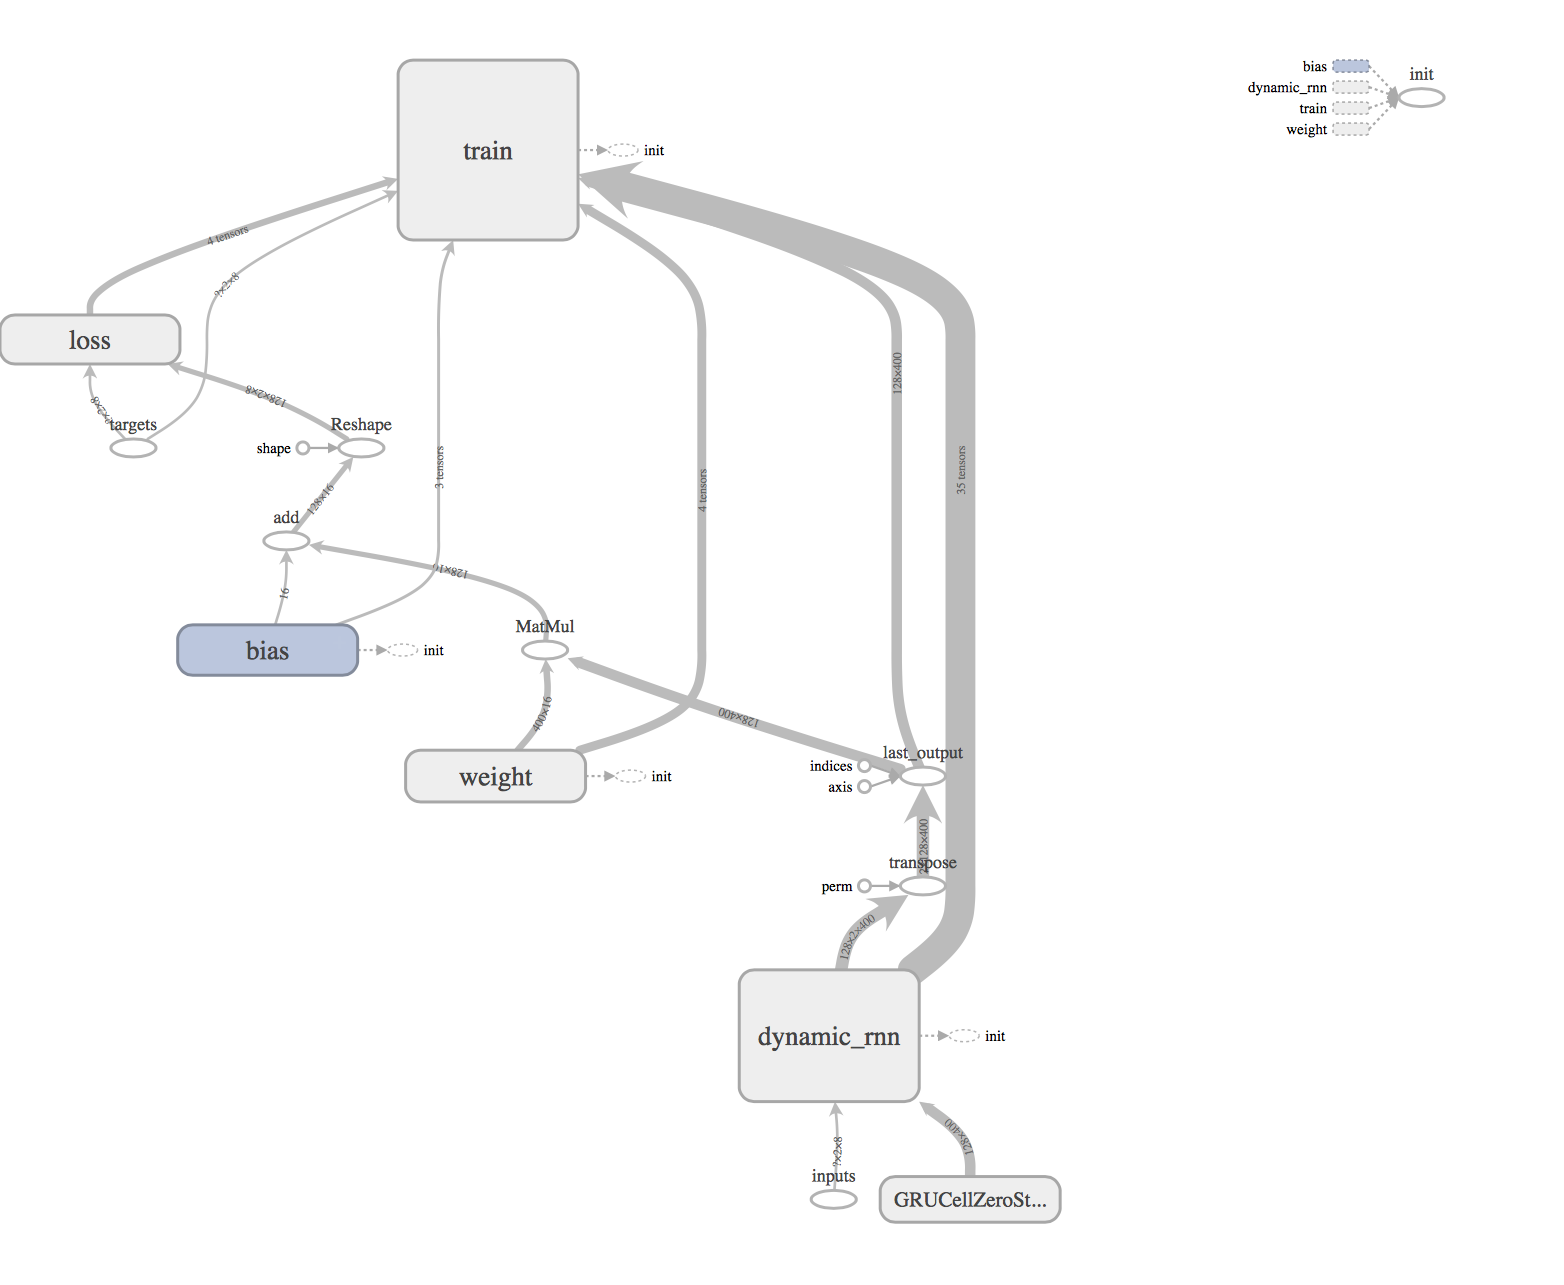
\includegraphics[width=\textwidth]{Figures/TF_graph.png}
    \caption[Network computation]{ Computation graph visualised using TensorBoard}

    \label{fig:tf_graph}
\end{figure}

Figure \ref{fig:tf_graph} represents the TensorFlow graph for computation of the model. In the top right, is the initialisation of the weights, biases in the model.

Loss is the sum of squared Euclidean errors. The hidden state of the GRU is saved and used for prediction.  % Evaluation

\chapter{Results and Discussion}


Future work would be to:
1. Combine states/ gait states , or have a first level classification of what state the pedestrian is : like stopping, starting, running, walking. 
2. A model that takes in as input the head pose orientation of the walking pedestrian
3. A system that talks with other identified components and contextual features 

About the window size.
About having a mechanism where more weight-age is given to the last point in the trajectory. 
About modelling uncertainty and thus getting better results
 % Results and Discussion

\chapter{Conclusion} % Conclusion

%\input{Chapters/Chapter7} % Conclusion

%% ----------------------------------------------------------------
% Now begin the Appendices, including them as separate files

\addtocontents{toc}{\vspace{2em}} % Add a gap in the Contents, for aesthetics

\appendix % Cue to tell LaTeX that the following 'chapters' are Appendices

\chapter{An Appendix}

Gosh is this counted in the word	% Appendix Title

%\input{Appendices/AppendixB} % Appendix Title

%\input{Appendices/AppendixC} % Appendix Title

\addtocontents{toc}{\vspace{2em}}  % Add a gap in the Contents, for aesthetics
\backmatter

%% ----------------------------------------------------------------
\label{Bibliography}
\lhead{\emph{Bibliography}}  % Change the left side page header to "Bibliography"
\bibliographystyle{unsrtnat}  % Use the "unsrtnat" BibTeX style for formatting the Bibliography
\bibliography{Bibliography}  % The references (bibliography) information are stored in the file named "Bibliography.bib"

\end{document}  % The End
%% ----------------------------------------------------------------